
 \begin{figure*}
 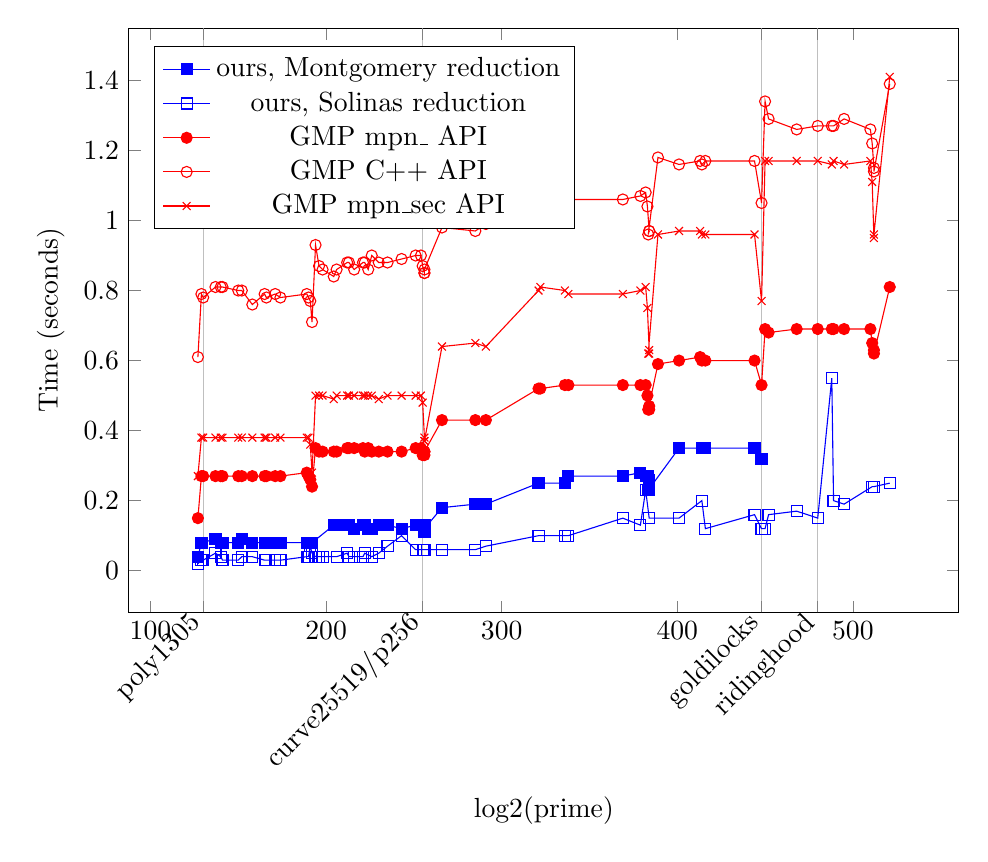
\begin{tikzpicture}
 	\begin{axis}[
 		height=9cm,
 		width=\textwidth,
 		legend pos= north west,
 		xtick distance=100,
 		extra x ticks={130,255,448,480},
 		extra x tick style={grid=major, tick label style={rotate=45,anchor=east}},
 		extra x tick labels={poly1305,curve25519/p256,goldilocks,ridinghood},
 		xlabel=log2(prime),
 		ylabel=Time (seconds)]		\addplot[color=blue,mark=square*] coordinates {
			(127.0, 0.04) 
			(129.0, 0.08) 
			(137.0, 0.09) 
			(140.0, 0.08) 
			(141.0, 0.08) 
			(150.0, 0.08) 
			(152.0, 0.09) 
			(158.0, 0.08) 
			(165.0, 0.08) 
			(166.0, 0.08) 
			(171.0, 0.08) 
			(174.0, 0.08) 
			(189.0, 0.08) 
			(190.0, 0.08) 
			(191.0, 0.08) 
			(192.0, 0.08) 
			(204.37503943134692, 0.13) 
			(206.0, 0.13) 
			(212.0, 0.13) 
			(213.0, 0.13) 
			(216.0, 0.12) 
			(221.0, 0.13) 
			(222.0, 0.13) 
			(224.0, 0.12) 
			(226.0, 0.12) 
			(230.0, 0.13) 
			(235.0, 0.13) 
			(243.0, 0.12) 
			(251.0, 0.13) 
			(253.98877343250717, 0.13) 
			(255.0, 0.13) 
			(256.0, 0.13) 
			(255.99999999966408, 0.11) 
			(255.9980614856364, 0.12) 
			(266.0, 0.18) 
			(285.0, 0.19) 
			(291.0, 0.19) 
			(321.0, 0.25) 
			(336.0, 0.25) 
			(338.0, 0.27) 
			(369.0, 0.27) 
			(379.0, 0.28) 
			(382.0, 0.27) 
			(383.0, 0.27) 
			(384.0, 0.26) 
			(383.9998899269044, 0.23) 
			(383.467605550083, 0.23) 
			(401.0, 0.35) 
			(414.0, 0.35) 
			(416.0, 0.35) 
			(444.0, 0.35) 
			(448.0, 0.32) 
		};
		\addlegendentry{ours, Montgomery reduction}

		\addplot[color=blue,mark=square] coordinates {
			(127.0, 0.02) 
			(129.0, 0.03) 
			(130.0, 0.03) 
			(137.0, 0.05) 
			(140.0, 0.04) 
			(141.0, 0.03) 
			(150.0, 0.03) 
			(152.0, 0.04) 
			(158.0, 0.04) 
			(165.0, 0.03) 
			(166.0, 0.03) 
			(171.0, 0.03) 
			(174.0, 0.03) 
			(189.0, 0.04) 
			(190.0, 0.04) 
			(191.0, 0.07) 
			(192.0, 0.05) 
			(194.0, 0.04) 
			(196.0, 0.04) 
			(198.0, 0.04) 
			(206.0, 0.04) 
			(212.0, 0.05) 
			(213.0, 0.04) 
			(216.0, 0.04) 
			(221.0, 0.04) 
			(222.0, 0.05) 
			(226.0, 0.04) 
			(230.0, 0.05) 
			(235.0, 0.07) 
			(243.0, 0.10) 
			(251.0, 0.06) 
			(255.0, 0.06) 
			(256.0, 0.06) 
			(266.0, 0.06) 
			(285.0, 0.06) 
			(291.0, 0.07) 
			(321.0, 0.10) 
			(336.0, 0.10) 
			(338.0, 0.10) 
			(369.0, 0.15) 
			(379.0, 0.13) 
			(382.0, 0.23) 
			(384.0, 0.15) 
			(401.0, 0.15) 
			(414.0, 0.20) 
			(416.0, 0.12) 
			(444.0, 0.16) 
			(448.0, 0.12) 
			(450.0, 0.12) 
			(452.0, 0.16) 
			(468.0, 0.17) 
			(480.0, 0.15) 
			(488.0, 0.55) 
			(489.0, 0.20) 
			(495.0, 0.19) 
			(511.0, 0.24) 
			(512.0, 0.24) 
			(521.0, 0.25) 
		};
		\addlegendentry{ours, Solinas reduction}

		\addplot[color=red,mark=*] coordinates {
			(127.0, 0.15) 
			(129.0, 0.27) 
			(130.0, 0.27) 
			(137.0, 0.27) 
			(140.0, 0.27) 
			(141.0, 0.27) 
			(150.0, 0.27) 
			(152.0, 0.27) 
			(158.0, 0.27) 
			(165.0, 0.27) 
			(166.0, 0.27) 
			(171.0, 0.27) 
			(174.0, 0.27) 
			(189.0, 0.28) 
			(190.0, 0.27) 
			(191.0, 0.26) 
			(192.0, 0.24) 
			(194.0, 0.35) 
			(196.0, 0.34) 
			(198.0, 0.34) 
			(204.37503943134692, 0.34) 
			(206.0, 0.34) 
			(212.0, 0.35) 
			(213.0, 0.35) 
			(216.0, 0.35) 
			(221.0, 0.35) 
			(222.0, 0.34) 
			(224.0, 0.35) 
			(226.0, 0.34) 
			(230.0, 0.34) 
			(235.0, 0.34) 
			(243.0, 0.34) 
			(251.0, 0.35) 
			(253.98877343250717, 0.35) 
			(255.0, 0.33) 
			(256.0, 0.34) 
			(255.99999999966408, 0.33) 
			(255.9980614856364, 0.34) 
			(266.0, 0.43) 
			(285.0, 0.43) 
			(291.0, 0.43) 
			(321.0, 0.52) 
			(322.0, 0.52) 
			(336.0, 0.53) 
			(338.0, 0.53) 
			(369.0, 0.53) 
			(379.0, 0.53) 
			(382.0, 0.53) 
			(383.0, 0.50) 
			(384.0, 0.47) 
			(383.9998899269044, 0.46) 
			(383.467605550083, 0.46) 
			(389.0, 0.59) 
			(401.0, 0.60) 
			(413.0, 0.61) 
			(414.0, 0.60) 
			(416.0, 0.60) 
			(444.0, 0.60) 
			(448.0, 0.53) 
			(450.0, 0.69) 
			(452.0, 0.68) 
			(468.0, 0.69) 
			(480.0, 0.69) 
			(488.0, 0.69) 
			(489.0, 0.69) 
			(495.0, 0.69) 
			(509.97423531735535, 0.69) 
			(511.0, 0.65) 
			(511.9891505409899, 0.63) 
			(512.0, 0.62) 
			(521.0, 0.81) 
		};
		\addlegendentry{GMP mpn\_ API}

		\addplot[color=red,mark=o] coordinates {
			(127.0, 0.61) 
			(129.0, 0.79) 
			(130.0, 0.78) 
			(137.0, 0.81) 
			(140.0, 0.81) 
			(141.0, 0.81) 
			(150.0, 0.80) 
			(152.0, 0.80) 
			(158.0, 0.76) 
			(165.0, 0.79) 
			(166.0, 0.78) 
			(171.0, 0.79) 
			(174.0, 0.78) 
			(189.0, 0.79) 
			(190.0, 0.78) 
			(191.0, 0.77) 
			(192.0, 0.71) 
			(194.0, 0.93) 
			(196.0, 0.87) 
			(198.0, 0.86) 
			(204.37503943134692, 0.84) 
			(206.0, 0.86) 
			(212.0, 0.88) 
			(213.0, 0.88) 
			(216.0, 0.86) 
			(221.0, 0.88) 
			(222.0, 0.88) 
			(224.0, 0.86) 
			(226.0, 0.90) 
			(230.0, 0.88) 
			(235.0, 0.88) 
			(243.0, 0.89) 
			(251.0, 0.90) 
			(253.98877343250717, 0.90) 
			(255.0, 0.87) 
			(256.0, 0.85) 
			(255.99999999966408, 0.85) 
			(255.9980614856364, 0.86) 
			(266.0, 0.98) 
			(285.0, 0.97) 
			(291.0, 0.99) 
			(321.0, 1.16) 
			(322.0, 1.13) 
			(336.0, 1.07) 
			(338.0, 1.06) 
			(369.0, 1.06) 
			(379.0, 1.07) 
			(382.0, 1.08) 
			(383.0, 1.04) 
			(384.0, 0.97) 
			(383.9998899269044, 0.97) 
			(383.467605550083, 0.96) 
			(389.0, 1.18) 
			(401.0, 1.16) 
			(413.0, 1.17) 
			(414.0, 1.16) 
			(416.0, 1.17) 
			(444.0, 1.17) 
			(448.0, 1.05) 
			(450.0, 1.34) 
			(452.0, 1.29) 
			(468.0, 1.26) 
			(480.0, 1.27) 
			(488.0, 1.27) 
			(489.0, 1.27) 
			(495.0, 1.29) 
			(509.97423531735535, 1.26) 
			(511.0, 1.22) 
			(511.9891505409899, 1.15) 
			(512.0, 1.14) 
			(521.0, 1.39) 
		};
		\addlegendentry{GMP C++ API}

		\addplot[color=red,mark=x] coordinates {
			(127.0, 0.27) 
			(129.0, 0.38) 
			(130.0, 0.38) 
			(137.0, 0.38) 
			(140.0, 0.38) 
			(141.0, 0.38) 
			(150.0, 0.38) 
			(152.0, 0.38) 
			(158.0, 0.38) 
			(165.0, 0.38) 
			(166.0, 0.38) 
			(171.0, 0.38) 
			(174.0, 0.38) 
			(189.0, 0.38) 
			(190.0, 0.38) 
			(191.0, 0.36) 
			(192.0, 0.28) 
			(194.0, 0.50) 
			(196.0, 0.50) 
			(198.0, 0.50) 
			(204.37503943134692, 0.49) 
			(206.0, 0.50) 
			(212.0, 0.50) 
			(213.0, 0.50) 
			(216.0, 0.50) 
			(221.0, 0.50) 
			(222.0, 0.50) 
			(224.0, 0.50) 
			(226.0, 0.50) 
			(230.0, 0.49) 
			(235.0, 0.50) 
			(243.0, 0.50) 
			(251.0, 0.50) 
			(253.98877343250717, 0.50) 
			(255.0, 0.48) 
			(256.0, 0.38) 
			(255.99999999966408, 0.37) 
			(255.9980614856364, 0.37) 
			(266.0, 0.64) 
			(285.0, 0.65) 
			(291.0, 0.64) 
			(321.0, 0.80) 
			(322.0, 0.81) 
			(336.0, 0.80) 
			(338.0, 0.79) 
			(369.0, 0.79) 
			(379.0, 0.80) 
			(382.0, 0.81) 
			(383.0, 0.75) 
			(384.0, 0.63) 
			(383.9998899269044, 0.62) 
			(383.467605550083, 0.62) 
			(389.0, 0.96) 
			(401.0, 0.97) 
			(413.0, 0.97) 
			(414.0, 0.96) 
			(416.0, 0.96) 
			(444.0, 0.96) 
			(448.0, 0.77) 
			(450.0, 1.17) 
			(452.0, 1.17) 
			(468.0, 1.17) 
			(480.0, 1.17) 
			(488.0, 1.16) 
			(489.0, 1.17) 
			(495.0, 1.16) 
			(509.97423531735535, 1.17) 
			(511.0, 1.11) 
			(511.9891505409899, 0.95) 
			(512.0, 0.96) 
			(521.0, 1.41) 
		};
		\addlegendentry{GMP mpn\_sec API}

	\end{axis}
\end{tikzpicture}
\end{figure*}
